\documentclass[main.tex]{subfiles}
\begin{document}

\chapter{Bayesian Inference and Conjugate Priors}\label{ch:bayes}\chaptermark{Bayesian Inference}

In the chapters of the book so far, the parameter $\theta$ was an unknown but fixed number; probability described only the randomness of the data. The Bayesian approach expresses the uncertainty about the parameter by probability as well: before the data, our knowledge about $\theta$ is summarised by a \emph{prior\index{prior distribution@prior distribution}} distribution; after the data are observed, Bayes' formula\index{bayes formula@Bayes' formula} (Theorem~\ref{thm:bayes}) updates this knowledge to a \emph{posterior\index{posterior distribution@posterior distribution}} distribution. In this chapter we discuss the basic objects of Bayesian inference, the closed-form solutions given by conjugate\index{conjugate prior@conjugate prior} priors, the decision-theoretic foundation, and why Bayesian and frequentist results merge in large samples (Bernstein--von Mises\index{bernstein von mises theorem@Bernstein--von Mises theorem}). For non-conjugate models we also implement the simplest example of Markov chain Monte Carlo (MCMC\index{mcmc@MCMC}).

\section{Definitions}

\begin{definition}[Prior, Likelihood, Posterior]\index{posterior distribution@posterior distribution|textbf}\index{prior distribution@prior distribution|textbf}
Let $\pi(\theta)$ be the \emph{prior} density of $\theta$ and $f(\x\mid\theta)=L(\theta;\x)$ the conditional density of the data. By Bayes' theorem the \emph{posterior} density is
\[
\pi(\theta\mid\x)=\frac{f(\x\mid\theta)\pi(\theta)}{m(\x)},\qquad m(\x)=\int_\Theta f(\x\mid\theta)\pi(\theta)\,d\theta .
\]
$m(\x)$ is called the \emph{marginal likelihood} (evidence). In short: $\text{posterior}\propto\text{likelihood}\times\text{prior}$.
\end{definition}

\begin{definition}[Conjugate Prior Family]\index{conjugate prior@conjugate prior|textbf}\index{prior distribution@prior distribution|textbf}
Let $\mathcal P$ be a family of priors. If $\pi(\cdot\mid\x)\in\mathcal P$ for every $\pi\in\mathcal P$ and every $\x$, then $\mathcal P$ is \emph{conjugate} for the model $\{f(\cdot\mid\theta)\}$.
\end{definition}

\begin{definition}[Posterior Predictive Distribution]\index{posterior distribution@posterior distribution|textbf}
For a new observation $\tilde X$, $f(\tilde x\mid\x)=\int f(\tilde x\mid\theta)\pi(\theta\mid\x)\,d\theta$ is the \emph{posterior predictive\index{posterior predictive distribution@posterior predictive distribution} distribution}; it carries the parameter uncertainty into the prediction.
\end{definition}

\begin{definition}[Bayes Risk and Bayes Estimator]
For a loss $L(\theta,a)$ and risk $R(\theta,\delta)$ (Definition~\ref{def:risk}), the \emph{Bayes risk\index{bayes risk@Bayes risk}} is $r(\pi,\delta)=\int R(\theta,\delta)\pi(\theta)d\theta$. The $\delta^\pi$ minimising $r(\pi,\cdot)$ is called the \emph{Bayes estimator\index{bayes estimator@Bayes estimator}}. Since by Fubini $r(\pi,\delta)=\int\Big[\int L(\theta,\delta(\x))\pi(\theta\mid\x)d\theta\Big]m(\x)d\x$, $\delta^\pi(\x)$ is found by minimising the \emph{posterior expected loss} for each $\x$.
\end{definition}

\begin{definition}[Credible Interval and HPD Region]\index{hpd region@HPD region|textbf}
A set $C\subseteq\Theta$ with $\int_C\pi(\theta\mid\x)d\theta=1-\alpha$ is called a $1-\alpha$ \emph{credible} set. A credible set\index{credible interval@credible interval} of the form $C=\{\theta:\pi(\theta\mid\x)\ge k_\alpha\}$ is called a \emph{highest posterior density} (HPD) region; it is the smallest set with the given probability.
\end{definition}

\begin{definition}[Jeffreys Prior]\index{jeffreys prior@Jeffreys prior|textbf}\index{prior distribution@prior distribution|textbf}
$\pi_J(\theta)\propto\sqrt{I_1(\theta)}$ (in the multidimensional case $\sqrt{\det I_1(\bm\theta)}$). Its total integral may be infinite (an \emph{improper} prior); it can be used for inference as long as the posterior is proper.
\end{definition}

\section{Main Theorems and Proofs}

\begin{theorem}[Beta--Binomial Conjugacy]\label{thm:beta-binom}\index{conjugate prior@conjugate prior}
If $\theta\sim\text{Beta}(\alpha,\beta)$ and $X\mid\theta\sim\text{Bin}(n,\theta)$, then
\[
\theta \mid X=x \sim \text{Beta}(\alpha + x,\ \beta + n - x),\qquad \hat{\theta}_{\text{Bayes}} =\E[\theta\mid x]= \frac{\alpha + x}{\alpha + \beta + n}.
\]
\end{theorem}
\begin{proof}
$\pi(\theta\mid x)\propto\theta^x(1-\theta)^{n-x}\cdot\theta^{\alpha-1}(1-\theta)^{\beta-1}=\theta^{\alpha+x-1}(1-\theta)^{\beta+n-x-1}$; up to the normalising constant this is the $\text{Beta}(\alpha+x,\beta+n-x)$ density. The mean of $\text{Beta}(a,b)$ is $a/(a+b)$.
\end{proof}

\begin{corollary}[Shrinkage Form]\label{cor:buzme}\index{shrinkage@shrinkage}
\[
\hat\theta_{\text{Bayes}}=\underbrace{\frac{\alpha+\beta}{\alpha+\beta+n}}_{w}\cdot\underbrace{\frac{\alpha}{\alpha+\beta}}_{\text{prior mean}}+\Big(1-w\Big)\cdot\underbrace{\frac{x}{n}}_{\text{MLE}} .
\]
The posterior\index{posterior distribution@posterior distribution} mean is a weighted average of the prior mean and the MLE. $\alpha+\beta$ acts like the ``equivalent sample size'' of the prior; as $n\to\infty$, $w\to0$ and the data dominate.
\end{corollary}
\begin{proof}
$\frac{\alpha+x}{\alpha+\beta+n}=\frac{\alpha+\beta}{\alpha+\beta+n}\cdot\frac{\alpha}{\alpha+\beta}+\frac{n}{\alpha+\beta+n}\cdot\frac xn$ and $\frac{n}{\alpha+\beta+n}=1-w$.
\end{proof}

\begin{theorem}[Bayes Estimators for Different Loss Functions]\label{thm:bayes-tahmin}
\begin{enumerate}
  \item Squared loss $L=(\theta-a)^2$: $\delta^\pi(\x)=\E[\theta\mid\x]$ (the posterior mean).
  \item Absolute loss $L=|\theta-a|$: $\delta^\pi(\x)=$ the posterior median.
  \item The limit of 0--1 loss ($L=\I\{|\theta-a|>\varepsilon\}$, $\varepsilon\to0$): the posterior mode (MAP).
\end{enumerate}
\end{theorem}
\begin{proof}
(1) Under the posterior, $\E[(\theta-a)^2\mid\x]=\Var(\theta\mid\x)+(\E[\theta\mid\x]-a)^2$ (exactly as in Theorem~\ref{thm:mse-ayrisim}); this is smallest at $a=\E[\theta\mid\x]$.
(2) For $g(a)=\E|\theta-a|$, $g'(a)=\P(\theta<a\mid\x)-\P(\theta>a\mid\x)$, which changes sign at the median.
(3) $\E[L]=1-\P(|\theta-a|\le\varepsilon\mid\x)\approx1-2\varepsilon\,\pi(a\mid\x)$; the $a$ at which the density is largest is chosen.
\end{proof}

\begin{theorem}[Normal--Normal Conjugacy]\label{thm:normal-normal}\index{conjugate prior@conjugate prior}
If $\theta\sim\Normal(\mu_0,\tau^2)$ and $X_i\mid\theta\iid\Normal(\theta,\sigma^2)$ ($\sigma^2$ known), then
\[
\theta\mid\x\sim\Normal(\mu_n,\tau_n^2),\qquad\frac{1}{\tau_n^2}=\frac1{\tau^2}+\frac{n}{\sigma^2},\qquad\mu_n=\tau_n^2\Big(\frac{\mu_0}{\tau^2}+\frac{n\bar x}{\sigma^2}\Big).
\]
\end{theorem}
\begin{proof}
The terms depending on $\theta$: $\ln\pi(\theta\mid\x)=-\frac{(\theta-\mu_0)^2}{2\tau^2}-\frac{n(\bar x-\theta)^2}{2\sigma^2}+\text{const}$ (because $\sum(x_i-\theta)^2=\sum(x_i-\bar x)^2+n(\bar x-\theta)^2$). The coefficient of $\theta^2$ is $-\frac12(1/\tau^2+n/\sigma^2)=-\frac1{2\tau_n^2}$ and that of $\theta$ is $\mu_0/\tau^2+n\bar x/\sigma^2=\mu_n/\tau_n^2$; completing the square gives $-\frac{(\theta-\mu_n)^2}{2\tau_n^2}+\text{const}$.
\end{proof}

\begin{remark}
Precisions (inverse variances) add: $\text{posterior precision}=\text{prior precision}+\text{data precision}$. The posterior mean is the precision-weighted average. This structure is the essence of the Kalman filter and of hierarchical (multilevel) models.
\end{remark}

\begin{theorem}[Gamma--Poisson Conjugacy]\label{thm:gamma-poisson}\index{conjugate prior@conjugate prior}
If $\lambda\sim\text{Gamma}(\alpha,\beta)$ (shape, rate) and $X_i\mid\lambda\iid\text{Poisson}(\lambda)$, then $\lambda\mid\x\sim\text{Gamma}(\alpha+\sum x_i,\ \beta+n)$. The posterior mean is $\frac{\alpha+\sum x_i}{\beta+n}$; the posterior predictive\index{posterior predictive distribution@posterior predictive distribution} distribution of a new observation is negative binomial (compare with Example~\ref{ex:poisson-gamma}).
\end{theorem}
\begin{proof}
$\pi(\lambda\mid\x)\propto\lambda^{\sum x_i}e^{-n\lambda}\cdot\lambda^{\alpha-1}e^{-\beta\lambda}$.
\end{proof}

\begin{theorem}[Invariance of the Jeffreys Prior \cite{jeffreys46}]\label{thm:jeffreys}\index{jeffreys prior@Jeffreys prior}\index{prior distribution@prior distribution}
If $\eta=h(\theta)$ is one-to-one and differentiable, the prior on $\eta$ obtained from the Jeffreys prior on the $\theta$ scale by a change of variables equals the Jeffreys prior defined directly on the $\eta$ scale.
\end{theorem}
\begin{proof}
Change of variables: $\pi(\eta)=\pi_J(\theta)\big|\frac{d\theta}{d\eta}\big|\propto\sqrt{I^{(\theta)}(\theta)}\big|\frac{d\theta}{d\eta}\big|=\sqrt{I^{(\theta)}(\theta)\big(\frac{d\theta}{d\eta}\big)^2}=\sqrt{I^{(\eta)}(\eta)}$; the last step is Proposition~\ref{prop:yeniden-param}.
\end{proof}

\begin{theorem}[Bernstein--von Mises; see {\cite[Theorem~10.1]{vdv}}]\label{thm:bvm}\index{bernstein von mises theorem@Bernstein--von Mises theorem}
In a regular parametric model, for a prior that is continuous and positive at $\theta_0$, under the true $\theta_0$
\[
\sup_B\Big|\Pi\big(\theta\in B\mid\X\big)-\Normal\big(\hat\theta_n,\,I_n(\theta_0)^{-1}\big)(B)\Big|\pto0 .
\]
That is, in large samples the posterior approaches a normal distribution centred at the MLE with variance equal to the inverse Fisher information\index{fisher information@Fisher information}; the influence of the prior disappears and Bayesian credible intervals\index{credible interval@credible interval} also have $1-\alpha$ coverage in the frequentist sense.
\end{theorem}
\begin{remark}[About the Proof]
For a complete proof see \cite[Theorem~10.1 and Lemma~10.3]{vdv}; the proof has two components. (i) \emph{Local asymptotic normality\index{asymptotic normality@asymptotic normality}:} for the local parameter $h=\sqrt n(\theta-\theta_0)$, the Taylor expansion of the proof of Theorem~\ref{thm:mle-an} gives
\[
\ell\big(\theta_0+h/\sqrt n\big)-\ell(\theta_0)=h\Delta_n-\tfrac12I_1(\theta_0)h^2+o_P(1),\qquad\Delta_n=\tfrac1{\sqrt n}\ell'(\theta_0)\dto\Normal(0,I_1).
\]
The posterior density of $h$ is proportional to $\pi(\theta_0+h/\sqrt n)\exp\{\ell(\theta_0+h/\sqrt n)-\ell(\theta_0)\}$; since the prior is continuous and positive at $\theta_0$, it approaches the constant $\pi(\theta_0)$, and the remaining expression, after completing the square, is proportional to the $\Normal(\Delta_n/I_1,\,1/I_1)$ density. Since $\Delta_n/I_1=\sqrt n(\hat\theta_n-\theta_0)+o_P(1)$, this is the normal distribution in the theorem. (ii) \emph{Control of the tails:} the approximation above is uniform only for $|h|\le M$; to show that the posterior mass far from $\theta_0$ goes to zero, one uses the existence of tests that consistently separate $H_0:\theta=\theta_0$ from $|\theta-\theta_0|\ge\varepsilon$. This is the technical part of the proof.
\end{remark}

\begin{remark}[Admissibility]
Every Bayes estimator\index{bayes estimator@Bayes estimator} that is unique and has finite Bayes risk\index{bayes risk@Bayes risk} with respect to a proper prior is admissible\index{admissibility@admissibility} (Definition~\ref{def:risk}): if there were a better estimator, its Bayes risk would also be smaller. Conversely (Wald's complete class theorem), every admissible estimator is a limit of Bayes estimators. This is the deep connection between frequentist optimality and Bayesian methods; the James--Stein\index{james stein estimator@James--Stein estimator} estimator (Chapter~\ref{ch:nokta-tahmin}) also has an empirical Bayes interpretation.
\end{remark}

\section{Worked Examples}

\begin{example}[Beta--Binomial: A Numerical Example]\label{ex:beta-binom-sayisal}
Earlier studies of the prevalence of a disease suggest a prior\index{prior distribution@prior distribution} with mean $0.10$: $\theta\sim\text{Beta}(2,18)$ (equivalent sample size $\alpha+\beta=20$). In a new screening, $x=10$ of $n=50$ people test positive (MLE $0.20$). The posterior\index{posterior distribution@posterior distribution} is $\text{Beta}(12,58)$ and
\[
\hat\theta_{\text{Bayes}}=\frac{12}{70}\approx0.171=\frac{20}{70}(0.10)+\frac{50}{70}(0.20).
\]
The posterior lies between the prior and the data, closer to the data.
\end{example}

\begin{example}[Posterior Prediction: Beta--Binomial]
In the same model, the probability that a new person tests positive is $\P(\tilde X=1\mid x)=\E[\theta\mid x]=\frac{\alpha+x}{\alpha+\beta+n}$. The posterior predictive\index{posterior predictive distribution@posterior predictive distribution} distribution of the number of positives among $m$ new people is \emph{beta-binomial}:
\[
\P(\tilde Y=k\mid x)=\binom mk\frac{B(\alpha+x+k,\ \beta+n-x+m-k)}{B(\alpha+x,\ \beta+n-x)},
\]
and its variance is larger than that of the binomial with the same mean: the parameter uncertainty carries over into the prediction.
\end{example}

\begin{example}[Laplace's Rule of Succession and the Jeffreys Prior]
For the Bernoulli, $I_1(\theta)=\frac{1}{\theta(1-\theta)}$, so $\pi_J(\theta)\propto\theta^{-1/2}(1-\theta)^{-1/2}$, i.e.\ $\text{Beta}(\frac12,\frac12)$. With the uniform prior $\text{Beta}(1,1)$ the posterior mean is $\frac{x+1}{n+2}$ (Laplace's rule of succession: ``if the sun has risen on $n$ days, the probability that it rises tomorrow is $\frac{n+1}{n+2}$''); with Jeffreys\index{jeffreys prior@Jeffreys prior} it is $\frac{x+1/2}{n+1}$. The equal-tailed interval obtained from the Jeffreys posterior is a binomial interval with very good frequentist coverage \cite{brown-cai}; it is examined in the code below.
\end{example}

\begin{example}[Normal--Normal: School Performance]
In an examination, school means are distributed as $\theta\sim\Normal(500,50^2)$. For one school, the mean of $n=25$ students is $\bar x=560$, with individual standard deviation $\sigma=100$ (so $\sigma^2/n=400$). Precisions: prior $1/2500$, data $1/400$. $\tau_n^2=1/(1/2500+1/400)\approx344.8$, $\tau_n\approx18.6$ and
\[
\mu_n=344.8\Big(\frac{500}{2500}+\frac{560}{400}\Big)\approx551.7 .
\]
The observed mean ``shrinks'' by $\approx8$ points towards the overall mean. This shrinkage\index{shrinkage@shrinkage}, which keeps schools with small samples from looking extremely good or bad, is standard practice in rankings in education and health (e.g.\ hospital mortality rates).
\end{example}

\begin{example}[Lindley's Paradox \cite{lindley57}]
$X_i\iid\Normal(\theta,1)$, $H_0:\theta=0$; prior $\P(H_0)=\frac12$ and $\theta\sim\Normal(0,1)$ under $H_1$. Suppose $\bar x=1.96/\sqrt n$ is observed (the $p$-value is $0.05$ for every $n$). The Bayes factor\index{bayes factor@Bayes factor} is
\[
B_{01}=\frac{\varphi(\bar x;0,1/n)}{\varphi(\bar x;0,1+1/n)}=\sqrt{n+1}\;\exp\Big\{-\frac{1.96^2}{2}\cdot\frac{n}{n+1}\Big\}\xrightarrow{n\to\infty}\infty .
\]
For $n=10\,000$, $B_{01}\approx15$ and $\P(H_0\mid\x)\approx0.94$: while the frequentist test rejects $H_0$ at the $5\%$ level, the posterior probability strongly supports $H_0$. The paradox arises because a fixed $p$-value corresponds to a very small effect size for large $n$.
\end{example}

\section{Computational Applications}

\subsection{Beta--Binomial: Posterior Summaries and the HPD Interval}

\pycode{code/ch19/c19_1_beta_binomial_posterior_summaries_hpd.py}
\begin{lstlisting}[style=output]
Bayes estimate: 0.1714
Credible interval: [0.09322494 0.2673681 ]
Posterior median = 0.1683 | mode (MAP) = 0.1618 | sd = 0.0447
95% HPD = [0.0879, 0.2603] (length 0.1724) | density at endpoints: 1.352, 1.352
Equal-tailed length = 0.1741
P(theta > 0.15 | x) = 0.6631
\end{lstlisting}

At the endpoints of the HPD\index{hpd region@HPD region} interval the posterior\index{posterior distribution@posterior distribution} density is equal (the Bayesian counterpart of Theorem~\ref{thm:en-kisa}), and the interval is slightly shorter than the equal-tailed one.

\subsection{Prior, Likelihood and Posterior; Bernstein--von Mises}

\pycode{code/ch19/c19_2_prior_likelihood_posterior_bvm.py}
\begin{lstlisting}[style=output]
n=   20 | posterior mean=0.1750 | MLE=0.2500 | TV(posterior, BvM normal)=0.4203
n=  200 | posterior mean=0.2091 | MLE=0.2200 | TV(posterior, BvM normal)=0.1658
n= 2000 | posterior mean=0.2178 | MLE=0.2190 | TV(posterior, BvM normal)=0.0550
\end{lstlisting}

\begin{figure}[h]
\centering
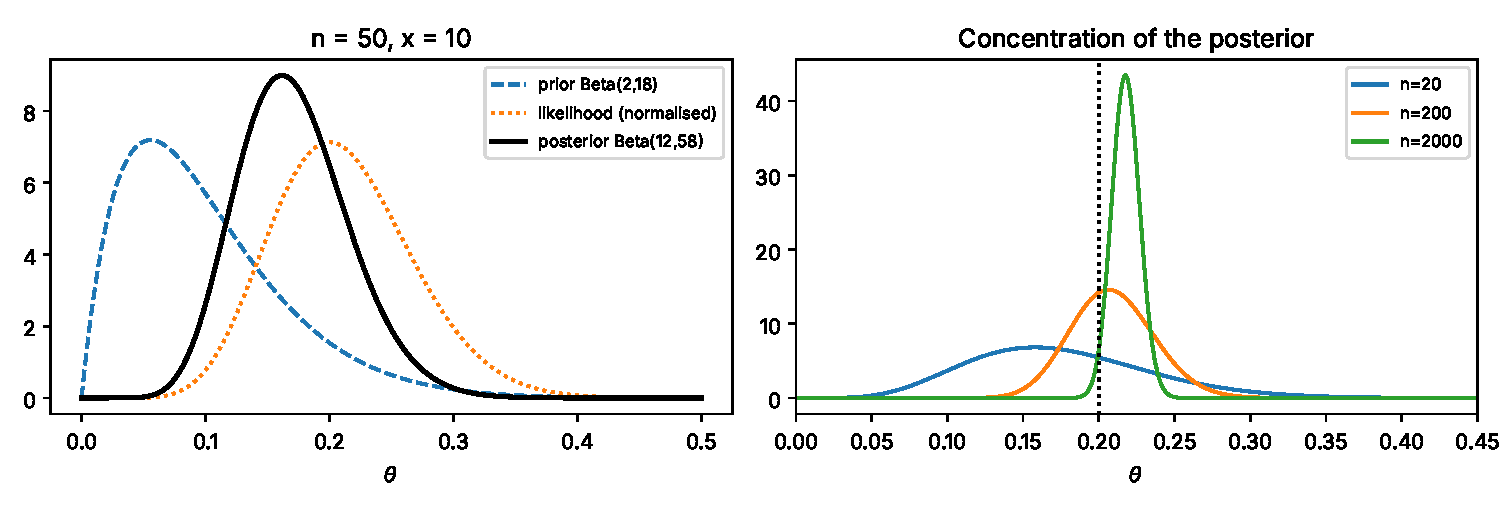
\includegraphics[width=\textwidth]{figures/bayes_sonsal.pdf}
\caption{Left: the posterior is a ``compromise'' between the prior and the likelihood. Right: as $n$ grows, the posterior concentrates around the true value $\theta_0=0.2$ and converges to the normal approximation (Bernstein--von Mises); the initial pull of the prior towards $0.1$ disappears.}
\end{figure}

\subsection{Frequentist Coverage of Bayesian Intervals}

\pycode{code/ch19/c19_3_frequentist_coverage_bayesian_intervals.py}
\begin{lstlisting}[style=output]
n= 30 | Jeffreys interval: mean coverage=0.9505, min=0.8887
n=100 | Jeffreys interval: mean coverage=0.9498, min=0.8806
\end{lstlisting}

The average frequentist coverage of the Jeffreys\index{jeffreys prior@Jeffreys prior} credible interval\index{credible interval@credible interval} is very close to the nominal level and clearly better than that of the Wald interval\index{wald confidence interval@Wald confidence interval} of Chapter~\ref{ch:guven}: well-chosen ``non-informative'' priors\index{prior distribution@prior distribution} produce methods with good frequentist properties.

\subsection{A Non-Conjugate Model: The Metropolis Algorithm}
The algorithm goes back to Metropolis\index{metropolis algorithm@Metropolis algorithm} and co-authors \cite{metropolis53}. If a $\Normal(0,1.5^2)$ prior is placed on the logit parameter $\eta=\ln\frac{\theta}{1-\theta}$, the posterior is not in closed form. The random-walk Metropolis algorithm: from the current $\eta$, propose $\eta'=\eta+\varepsilon$, $\varepsilon\sim\Normal(0,s^2)$; accept with probability $\min\{1,\pi(\eta'\mid x)/\pi(\eta\mid x)\}$. The stationary distribution of this chain is the posterior; the normalising constant $m(x)$ is never needed.

\pycode{code/ch19/c19_4_nonconjugate_model_metropolis.py}
\begin{lstlisting}[style=output]
Acceptance rate = 0.538
MCMC  posterior mean E[theta|x] = 0.2115 | 95% interval = [0.1126 0.3318]
Exact posterior mean (quad)      = 0.2119
Comparison: Beta(2,18) conjugate posterior mean = 0.1714 | MLE = 0.2000
\end{lstlisting}

The MCMC\index{mcmc@MCMC} estimate agrees to three digits with the exact value found by numerical integration. That the posterior mean now comes out \emph{above} the MLE is a consequence of the prior: the prior $\eta\sim\Normal(0,\,1.5^2)$ is centred at $\theta=0.5$ and pulls the posterior upwards, whereas the $\text{Beta}(2,18)$ prior, centred at $0.1$, pulled it downwards. This difference, obtained with the same data and different priors, shows why prior sensitivity analysis matters in small samples.

\section{Comments and Notes}

\begin{remark}[Choosing the Prior]
Most criticism is directed at the subjectivity of the prior\index{prior distribution@prior distribution}. Practical answers: (i) \emph{Sensitivity analysis}: does the result change across reasonable priors? (ii) \emph{Weakly informative priors}: priors that keep the parameter on a plausible scale without dominating the data. (iii) \emph{Hierarchical models}: learning the prior parameters from the data as well (empirical or full Bayes). The Bernstein--von Mises\index{bernstein von mises theorem@Bernstein--von Mises theorem} theorem guarantees that in large samples (in regular models) the influence of the prior disappears; in small samples the prior acts as a \emph{regulariser} (ridge\index{ridge regression@ridge regression} regression is the MAP estimate under a normal prior).
\end{remark}

\begin{remark}[Credibility and Confidence]
A $95\%$ credible interval\index{credible interval@credible interval} permits the statement ``the (posterior\index{posterior distribution@posterior distribution}) probability that $\theta$ lies in this interval is $0.95$'' --- exactly the interpretation that most practitioners wrongly attach to a confidence interval. The price is stating the prior explicitly. The two approaches coincide numerically in large samples (BvM); they can diverge in small samples, for parameters on the boundary, and in high-dimensional problems.
\end{remark}

\begin{remark}[Computation]
Conjugate\index{conjugate prior@conjugate prior} priors provide closed forms, but most modern Bayesian analysis is done with MCMC\index{mcmc@MCMC} (Metropolis\index{metropolis algorithm@Metropolis algorithm}--Hastings, Gibbs, Hamiltonian Monte Carlo), variational approximations or the Laplace approximation. Probabilistic programming languages such as Stan, PyMC and NumPyro automate these algorithms. Diagnosing chain convergence ($\hat R$, effective sample size, trace plots) is an integral part of these methods.
\end{remark}

% --- CHAPTER SUMMARY ---
\section{Chapter Summary}
\begin{summary}
\begin{itemize}
  \item In Bayesian inference the posterior is proportional to the product of the likelihood and the prior. Uncertainty is expressed by a probability distribution over the parameter.
  \item Conjugate priors give closed-form posteriors: Beta--Binomial (Theorem~\ref{thm:beta-binom}), Normal--Normal (Theorem~\ref{thm:normal-normal}) and Gamma--Poisson (Theorem~\ref{thm:gamma-poisson}). The posterior mean is a weighted average of the prior mean and the MLE (Corollary~\ref{cor:buzme}).
  \item The Bayes estimator depends on the loss function (Theorem~\ref{thm:bayes-tahmin}): the posterior mean for squared loss, the posterior median for absolute loss, and the posterior mode for $0$--$1$ loss.
  \item The Jeffreys prior is invariant under reparametrisation (Theorem~\ref{thm:jeffreys}). By the Bernstein--von Mises theorem (Theorem~\ref{thm:bvm}), in large samples the posterior approaches $\Normal(\hat\theta_n,I_n^{-1})$ and the influence of the prior disappears.
  \item For point null hypotheses the $p$-value and the posterior probability can diverge sharply (Lindley's paradox). When there is no closed form, the posterior is sampled by MCMC methods such as Metropolis.
\end{itemize}
\end{summary}
% --- END OF CHAPTER SUMMARY ---

\paragraph{Further reading.} \cite{gelman}, \cite[Chapter~11]{wasserman}, \cite[Chapter~4]{lehmann-casella}; for asymptotic Bayesian theory, \cite[Chapter~10]{vdv}.

\section{Exercises}

\begin{exercise}\label{exr:19-1}
In the Gamma--Poisson model, write the posterior mean as a weighted average of the prior mean and $\bar x$. For $\alpha=2$, $\beta=1$ and $\sum_{i=1}^{10}x_i=34$, compute the posterior mean, the $95\%$ equal-tailed credible interval and the posterior predictive distribution of a new observation.
\hfill\hyperref[coz:19-1]{\footnotesize$\rightarrow$\,Solution}
\end{exercise}

\begin{exercise}\label{exr:19-2}
When both the normal mean and variance are unknown, show that under the (improper) prior $\pi(\mu,\sigma^2)\propto1/\sigma^2$ the marginal posterior of $\mu$ satisfies
\[
\frac{\mu-\bar x}{s/\sqrt n}\,\Big|\,\x\sim t_{n-1} .
\]
How does this result relate to the $t$ interval of Chapter~\ref{ch:guven}?
\hfill\hyperref[coz:19-2]{\footnotesize$\rightarrow$\,Solution}
\end{exercise}

\begin{exercise}\label{exr:19-3}
In the Normal--Normal model, compute the frequentist MSE of the posterior mean $\mu_n$ as a function of $\theta$ and compare it with the MSE of $\bar X$ ($\sigma^2/n$). For which values of $\theta$ is the Bayes estimator better?
\hfill\hyperref[coz:19-3]{\footnotesize$\rightarrow$\,Solution}
\end{exercise}

\begin{exercise}\label{exr:19-4}
In the Metropolis code, compare the acceptance rates and the autocorrelation of the chain for proposal scales $s\in\{0.05,\,0.6,\,5\}$. Estimate the effective sample size with the formula $N/(1+2\sum_k\rho_k)$.
\hfill\hyperref[coz:19-4]{\footnotesize$\rightarrow$\,Solution}
\end{exercise}

\chapterlinks{19}

\end{document}
